\chapter{Trapped electrons: the Poisson--Boltzmann model}
\label{ch:pb}

Of the electrons the pulse releases, the fast ones escape and the rest are trapped by the growing positive charge.
The trapped electrons thermalize quickly and form a hot, dense nanoplasma~\cite{ditmire1996,saalmann2006,fennel2010},
which
\begin{enumerate}
  \item \emph{screens} the ions: it neutralizes the core and reshapes the field that drives the explosion;
  \item \emph{ionizes} further by electron impact, at a rate set by its local density and temperature
    (Chapter~\ref{ch:coll});
  \item \emph{loses} electrons and energy as the well becomes shallower and the fastest electrons evaporate.
\end{enumerate}
With \opt{mcmd-electrons = pbgrid} (the default) the trapped electrons are a continuous density $n(\vect x)$ on a
three-dimensional grid that follows the sample.
Every \opt{mcmd-pb-interval} (0.2\,fs) the density is recomputed as the equilibrium distribution of $N$ classical
electrons at one temperature $T$, in the field of the ions and of the electrons themselves.
$T$ is not a parameter: it follows from the electrons' total energy, which is booked event by event.
The density gives the forces on the ions, the depth that decides whether a new electron escapes, the local density
for collisions, and the electrons that evaporate.
How it is discretized and solved is in Appendix~\ref{app:numerics}.
With \opt{mcmd-electrons = none} there is no cloud: every released electron leaves.

\section{Why a continuum, and why Boltzmann}

Three lengths decide the description: the sample radius $R$ (a few nm, growing), the Debye length
$\lambda_D = \sqrt{\varepsilon_0T/(e^2n)}$ (0.05--0.5\,nm for $n\sim10^2$--$10^3$\,nm$^{-3}$ and $T\sim10$--$100$\,eV), and
the interionic distance (0.1--0.2\,nm in the intact protein).
With $\lambda_D\ll R$ the electrons behave like a conductor: they screen the field inside the sample, leaving a
quasi-neutral core with the net positive charge in a thin outer layer~\cite{chen2016}.
This follows from the Poisson--Boltzmann equation; it does not follow from a prescribed electron profile.

A classical Boltzmann gas at one temperature rests on three assumptions:
\begin{enumerate}
  \item \emph{fast thermalization}: the electron--electron collision rate, $10^{15}$--$10^{16}$\,s$^{-1}$~\cite{nrl}, is
    faster than the explosion;
  \item \emph{no degeneracy}: the thermal wavelength $\lambda_{\mathrm{th}}\approx0.12$\,nm at 10\,eV gives
    $n\lambda_{\mathrm{th}}^3\lesssim1$ except in the deepest wells;
  \item \emph{mean field}: correlations beyond the mean field are neglected; bound states are the atomic Monte Carlo
    module's business.
\end{enumerate}
The electrons follow the ions on the scale of the inverse plasma frequency, $\omega_p^{-1}\lesssim0.1$\,fs, much
faster than the ions move, so the density can be recomputed as an equilibrium rather than integrated in time.

\section{The free energy}

In the mean-field approximation the Helmholtz free energy of $N$ classical electrons at temperature $T$, in the field
of fixed ions, is
\begin{equation}
  F[n] = -\!\int n\,\Phi\,\dd^3x
        + \frac12\iint n(\vect x)\,K(\vect x-\vect y)\,n(\vect y)\,\dd^3x\,\dd^3y
        + T\!\int n\Big[\ln\frac{n}{n_\ast}-1\Big]\dd^3x,\qquad \int n\,\dd^3x = N,
  \label{eq:F}
\end{equation}
with the ions' attraction $\Phi(\vect x) = \kc\sum_a q_a G_s(|\vect x-\vect x_a|)$, the electron--electron kernel
$K(\vect r) = \kc G_s(r)$, and the entropy of an ideal gas ($n_\ast$ only shifts $F$ by a constant).
It is the classical, local limit of Mermin's finite-temperature density-functional theory~\cite{mermin1965}, without
exchange and correlation.
Minimizing $F$ at fixed $N$ with a chemical potential $\mu$ gives
\begin{equation}
  n(\vect x) = n_\ast\,e^{(\mu - V(\vect x))/T},\qquad V = -\Phi + K*n,
  \label{eq:boltzmann}
\end{equation}
the Boltzmann factor of the self-consistent potential.
Since $\nabla^2(1/r) = -4\pi\delta$, this is the Poisson--Boltzmann equation
$\nabla^2V = 4\pi\kc(\tilde\rho_{\mathrm{ion}}-\tilde n)$, $n\propto e^{-V/T}$ (with smoothed sources), solved with
open boundaries.
Hot, the cloud follows the shallow total well over the whole sample; cold, it neutralizes the interior and leaves the
net charge in a sheath of thickness $\sim\lambda_D$ at the surface.

$F$ is strictly convex: the entropy has second variation $T/n>0$, the Hartree term is positive definite (its kernel's
Fourier transform $\hat K = (4\pi\kc/k^2)\,e^{-k^2s^2/4}$ is positive), and the ion term is linear.
There is exactly one minimizer, and the solver (Appendix~\ref{app:numerics}) converges to it from any positive starting
density.

\section{The smoothed Coulomb kernel}
\label{sec:kernel}

Every charge --- ions and electron cells --- is a Gaussian, and two Gaussians interact through
\begin{equation}
  G_s(r) = \frac{\mathrm{erf}(r/s)}{r},\qquad G_s(0) = \frac{2}{s\sqrt\pi},
\end{equation}
the splitting that also underlies Ewald summation~\cite{darden1993,essmann1995}.
$G_s$ equals $1/r$ to $10^{-7}$ beyond $4s$ and is finite at $r=0$ (Fig.~\ref{fig:kernel}).

\begin{figure}[t]
  \centering
  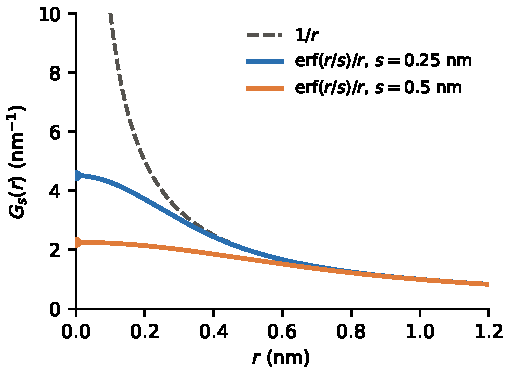
\includegraphics[width=0.5\textwidth]{fig/kernel.pdf}
  \caption{The smoothed Coulomb kernel $G_s(r) = \mathrm{erf}(r/s)/r$ against $1/r$; the dots are $G_s(0)$. The model's
  $s_e = 0.25$\,nm is the blue curve.}
  \label{fig:kernel}
\end{figure}

There are two reasons to smooth.
On a grid of spacing $\Delta x$ a cell is a blob of width $\sim\Delta x$; treating it as a Gaussian with $s=2\Delta x$
makes the grid sums smooth approximations of the integrals.
And physically, a classical Boltzmann gas collapses into a point ion ($e^{\kc q/rT}$ is not integrable at $r\to0$):
the electron's quantum size, 0.1--0.2\,nm at 10--50\,eV, blurs the singular well, and the bound part of the well is
the atomic module's.
The model uses
\begin{equation}
  s = \max\!\big(2\Delta x,\ s_e\big),\qquad s_e = \opt{mcmd-pb-smoothing} = 0.25\ \mathrm{nm},
\end{equation}
everywhere the kernel appears: the ion and electron potentials, the escape depth, distant ions and the long-range ion
force.
Once the grid resolves $s_e$ ($\Delta x\le s_e/2$), refining it no longer changes the physics.
The charge, the escape and the ion directions do not depend on $s_e$; the ion kinetic energy does
(Appendix~\ref{app:validation}).

\section{The temperature}
\label{sec:temperature}

The temperature is that of an ideal gas, $T = \frac23K/N$, with $K$ the electrons' kinetic energy --- the usual
equipartition definition, since the potential energy is explicit.
$K$ is not tracked directly: the model conserves the electrons' \emph{total} energy $E_{\mathrm{tot}} = K + U$, with
the electrostatic energy $U(\vect n) = \int n\,[-\Phi + \frac12K*n]$ (electrons with ions, and half their mutual
repulsion; the ion--ion energy is GROMACS's).
Since the density depends on $T$, $T$ and $\vect n$ are found together, from
\begin{equation}
  g(T) = E_{\mathrm{tot}} - U(\vect n_T) - \tfrac32NT = 0,
\end{equation}
where $\vect n_T$ minimizes $F$ at $T$.
A hotter cloud spreads into regions of higher potential energy, so $g$ decreases monotonically and has one root,
found by a safeguarded secant iteration (Appendix~\ref{app:numerics}).

\section{Energy bookkeeping}
\label{sec:energy}

Tracking $E_{\mathrm{tot}}$ instead of $K$ means that the adiabatic cooling of an expanding cloud, and the heating
when an ion's charge grows under it, appear by themselves in $K = E_{\mathrm{tot}} - U$.
$E_{\mathrm{tot}}$ changes only by explicit exchanges.
Write $V_e = K*n$ for the electrons' repulsion from the last solve, scaled by $\varsigma = N/N_{\mathrm{solve}}$ for
electrons added or lost since, and
\begin{equation}
  D_k = \kc\sum_{b\ne k} q_b\,G_s(|\vect x_k-\vect x_b|) - \varsigma\,V_e(\vect x_k)
  \label{eq:Dk}
\end{equation}
for the depth of the well at atom $k$: the binding energy of an electron at rest there.
\begin{enumerate}
  \item \textbf{Work on the ions.} The cloud's force on the ions does work $W$ per step, taken from the electrons:
    $\Delta E_{\mathrm{tot}} = -\sum_a\vect F_a\cdot\vect v_a\Delta t$.
  \item \textbf{A trapped photo- or Auger electron} of energy $\varepsilon$ at atom $k$:
    $\Delta E_{\mathrm{tot}} = \varepsilon - D_k$.
  \item \textbf{Collisional ionization} at $k$ with binding energy $\Delta E_{\mathrm b}$: a cloud electron pays it, and
    the freed electron starts at rest at $k$: $\Delta E_{\mathrm{tot}} = -\Delta E_{\mathrm b} - D_k$.
  \item \textbf{A change of an ion's charge} by $\Delta q$ changes its interaction with the cloud; the kinetic energy does
    not change at that instant: $\Delta E_{\mathrm{tot}} = -\Delta q\,\varsigma V_e(\vect x_k)$.
  \item \textbf{Evaporation} of $\delta N$ electrons with kinetic energy $\delta E$ from mean depth $\bar D$:
    $\Delta E_{\mathrm{tot}} = -(\delta E - \delta N\bar D)$.
  \item \textbf{A grid rebuild} changes $U$ for numerical reasons only; the change is moved into $E_{\mathrm{tot}}$ so
    that $K$ does not jump.
\end{enumerate}
An electron that escapes at birth never joins the cloud; it only raises the net charge.
\file{energy\_ledger.txt} and \file{pb\_log.txt} record these terms (Chapter~\ref{ch:output}).

\section{Forces on the ions}

An ion of charge $q_a$ has potential energy $-q_a\varsigma V_e(\vect x_a)$ in the cloud, so the cloud pulls on it with
\begin{equation}
  \vect F_a = q_a\,\varsigma\,\nabla V_e(\vect x_a),
\end{equation}
from central differences on the grid, interpolated to the atom (outside the grid: a point charge at the cloud's
centroid).
The forces are added to the GROMACS forces every step on every rank, and their work is booked (item~1).
Between solves the ions move through the fixed electron potential.

\section{Escape or trapping}
\label{sec:escape}

An electron of kinetic energy $\varepsilon$ released at atom $k$ escapes if $\varepsilon > D_k$ and is trapped
otherwise, with the depth~\eqref{eq:Dk} of the same smoothed ion potential and the same cloud the solve uses.
The atom's own new charge is left out: the electron leaves before the atom's remaining electrons rearrange.
An escaped electron adds one to the net charge $Q$; a trapped one adds one to $N$ and is booked as item~2.
Each electron is tested once, at birth: an escaped one cannot be recaptured, and a trapped one leaves only by
evaporation.

\section{Evaporation}
\label{sec:evaporation}

A well of finite depth cannot hold the tail of a Maxwell distribution: an electron whose kinetic energy exceeds its
local depth $D(\vect x) = -V(\vect x)$ is unbound and leaves, and collisions keep refilling the tail.
This evaporation (\opt{mcmd-evaporation = 1}, the default) matters late in the explosion, when the well is shallow and
the cloud still hot.
For a Maxwell distribution at $T$, the fraction of electrons above $D$ and the fraction of their kinetic energy above
$D$ are regularized incomplete gamma functions of $x = D/T$~\cite{abramowitz1964}:
\begin{equation}
  Q(\tfrac32,x) = \mathrm{erfc}\sqrt x + 2\sqrt{x/\pi}\,e^{-x},\qquad
  Q(\tfrac52,x) = Q(\tfrac32,x) + \tfrac{4}{3\sqrt\pi}x^{3/2}e^{-x}.
\end{equation}
The energy tail is the larger (Fig.~\ref{fig:tails}), so evaporation cools the cloud.
Summed over the cells of the last solve (binned by depth into 4000 bins once per solve),
$\delta N^{\mathrm{tail}} = \sum_i n_iQ(\frac32,x_i)$ and $\delta E^{\mathrm{tail}} = \frac32T\sum_in_iQ(\frac52,x_i)$.
The tail refills at the electron--electron collision rate~\cite{nrl}
\begin{equation}
  \nu_{ee} = 2.91\times10^{-6}\,n_e[\mathrm{cm^{-3}}]\,\ln\Lambda\,T^{-3/2}\ \mathrm{s^{-1}},\qquad
  \ln\Lambda = \max\big(2,\ 24-\ln(\sqrt{n_e}/T)\big),
\end{equation}
at the mean density $n_e = N/(\frac43\pi R^3)$, and every MD step a fraction $\phi = \min(1,\nu_{ee}\Delta t)$ of it
leaves: $N$ and $K$ fall by $\phi\varsigma\,\delta N^{\mathrm{tail}}$ and $\phi\varsigma\,\delta E^{\mathrm{tail}}$, the
net charge $Q$ rises, and the leavers' total energy is booked (item~5).
How many electrons evaporate depends on the box (Appendix~\ref{app:numerics}); the total that escapes, at birth and by
evaporation, does not.

\begin{figure}[t]
  \centering
  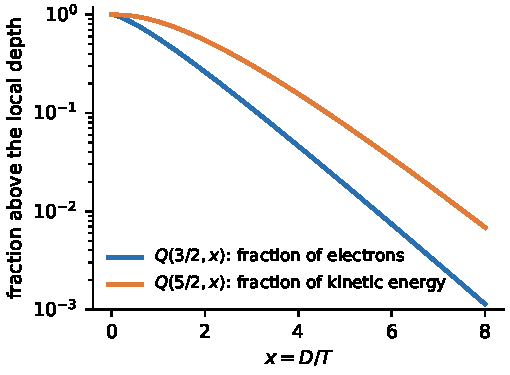
\includegraphics[width=0.5\textwidth]{fig/tails.pdf}
  \caption{The Maxwell tails above a depth $D$: the fraction of electrons $Q(\frac32,D/T)$ and of their kinetic energy
  $Q(\frac52,D/T)$.}
  \label{fig:tails}
\end{figure}

\section{Assumptions}

\begin{itemize}
  \item One temperature, instantaneous equilibrium: hot spots are averaged out at the next solve.
  \item Classical mean field: no degeneracy, exchange or correlation below the scale $s_e$; $s_e$ has a physical size
    but is not derived from first principles.
  \item Electrons frozen between solves (0.2\,fs), adequate while the ions move much less than a grid cell in that
    time.
  \item Escape at birth only; evaporation at the mean electron--electron collision rate, an estimate rather than a
    kinetic calculation.
  \item Far from the sample the cloud is a point charge.
\end{itemize}
